\documentclass{article}
\usepackage{graphicx} % Required for inserting images
\usepackage{hyperref}
\usepackage{amssymb}
\usepackage{amsmath}
\usepackage{amsthm}
\usepackage{geometry}

\newtheorem{lemma}{Lemma}
\newtheorem{method}{Method}
\newtheorem{definition}{Definition}
\newtheorem{theorem}{\bf Theorem}
\newtheorem{prop}{\bf Proposition}
\newtheorem{example}{Example}
\newtheorem{sol}{Solution}
\newtheorem{corollary}{Corollary}


\title{\vspace{-2cm} Split Graph}
\author{YF}
\date{November 2023}

\begin{document}

\maketitle
\hrule
\begin{definition}
    Split Graph
    
    A graph is called a split graph if its vertices can be split into one independent subgraph and one clique.
\end{definition}

\begin{theorem}
    A graph $G$ is split if and only if $G\in\text{Free}\{2K^2,\,C^4,\,C^5\}$.
\end{theorem}


    The '$\Rightarrow$' is clear, we need to show '$\Leftarrow$'. Suppose $2K^2$, $C^4$ and $C^5$ are not induced subgraph of $G$. Then take the largest clique $A$ and let $B=V(G)-A$. \\

    If vertices in $B$ are all disjoint, then the proof is done. If there are two vertices $v$ and $w$ that are adjacent, consider their neighborhoods in $A$, i.e. $N_A(v)=N(v)\cup A$ and $N_A(w)=N(w)\cup A$. It is clear that $N_A(v)\neq A$ and $N_A(w)\neq A$. Otherwise, we can take $v$ or $w$ into $A$ and form a larger clique, which gives a contradiction to the assumption of $A$. To prove '$\Leftarrow$', we try to find some properties for $G\in\text{Free}\{2K^2,\,C^4,\,C^5\}$ first.


    \begin{prop}\label{p2}
        One of the neighborhoods in $A$ of adjacent vertices is contained in another
    \end{prop}

    \begin{proof}
        Suppose $N_A(v)-N_A(v)\neq\emptyset$ and $N_A(w)-N_A(w)\neq\emptyset$, then take $a\in N_A(v)-N_A(v)$ and $b\in N_A(w)-N_A(w)$. Then $avwb$ is a $C^4$ which gives a contradiction to our assumption. Thus we know that
    \begin{equation*}
        N_A(v)\subseteq N_A(w)\ \vee\ N_A(w)\subseteq N_A(v)
    \end{equation*}
    \begin{figure}[h!]%靠文字内容的右侧
        \centering
        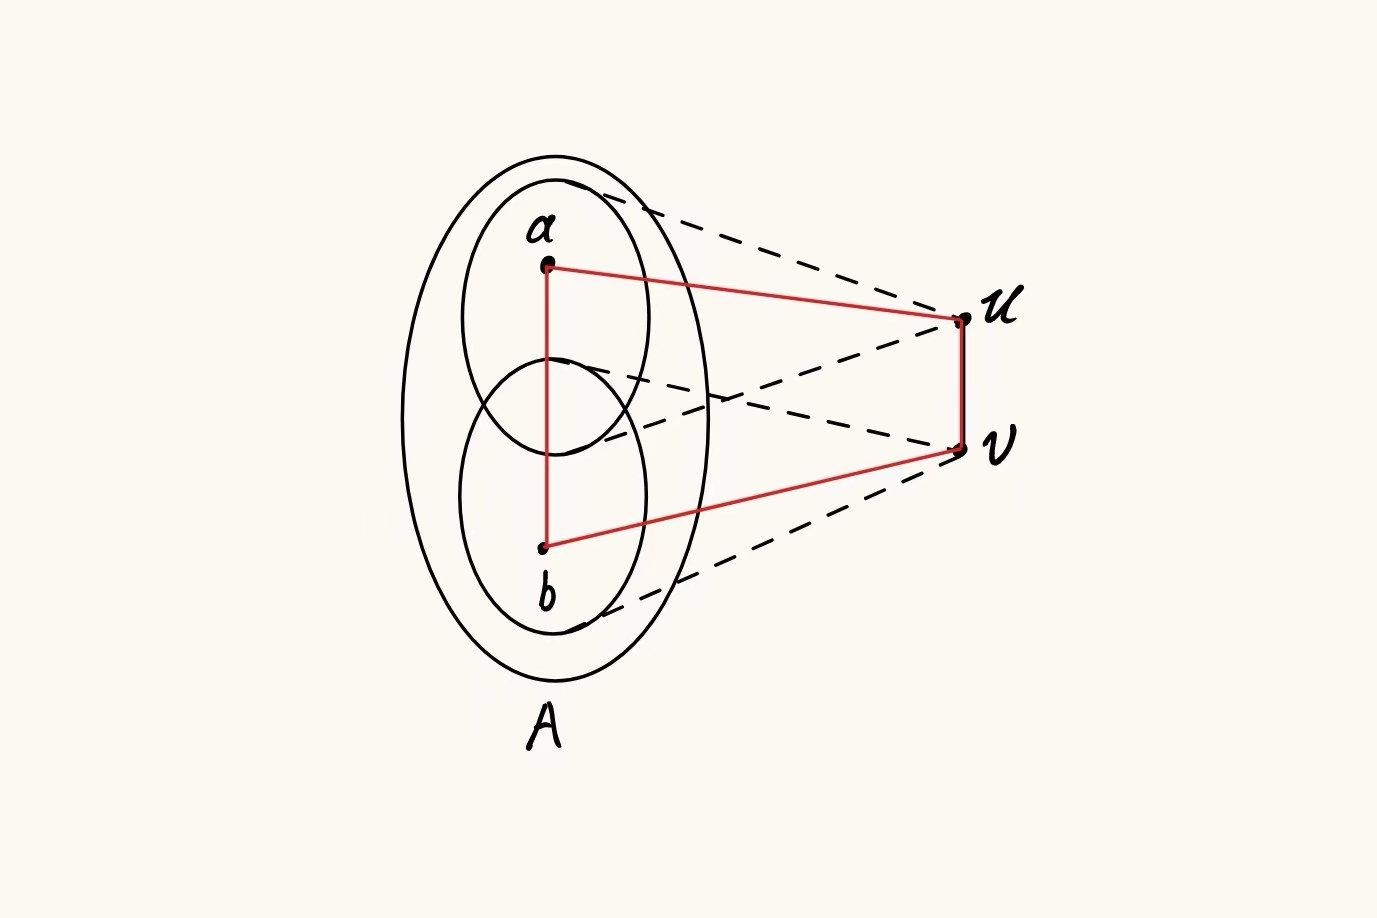
\includegraphics[width=0.45\textwidth]{pic/g1.jpg}
        %\caption{\textit{Schematic diagram of Hall effect}}\label{fig1}
\end{figure}
    \end{proof}

    
    \begin{prop}\label{p1}
        There is exactly one vertex out of $N_A(v)\cup N_A(w)$ in $A$ where $u$ and $v$ are adjacent.
    \end{prop}

    \begin{proof}
        By proposition\eqref{p2} and previous observation, we know that there should be at least one vertex out of $N_A(v)\cup N_A(w)$ Since 
        \begin{equation*}
            \begin{split}
                &N_A(v)\cup N_A(w)=N_A(v)\text{ or }N_A(w)\\
                &N_A(v)\neq A\neq N_A(w)
            \end{split}
        \end{equation*}        
        Now we prove the uniqueness. Suppose $\exists a,\,b\in A-(N_A(v)\cup N_A(w))$, then $ab+vw$ is a $2K^2$, which gives a contradiction to $G\in\text{Free}\{2K^2,\,C^4,\,C^5\}$. Then there is exactly one vertex in $A-N_A(v)\cup N_A(w)$, denoted by $k$.
        \begin{figure}[h!]%靠文字内容的右侧
            \centering
            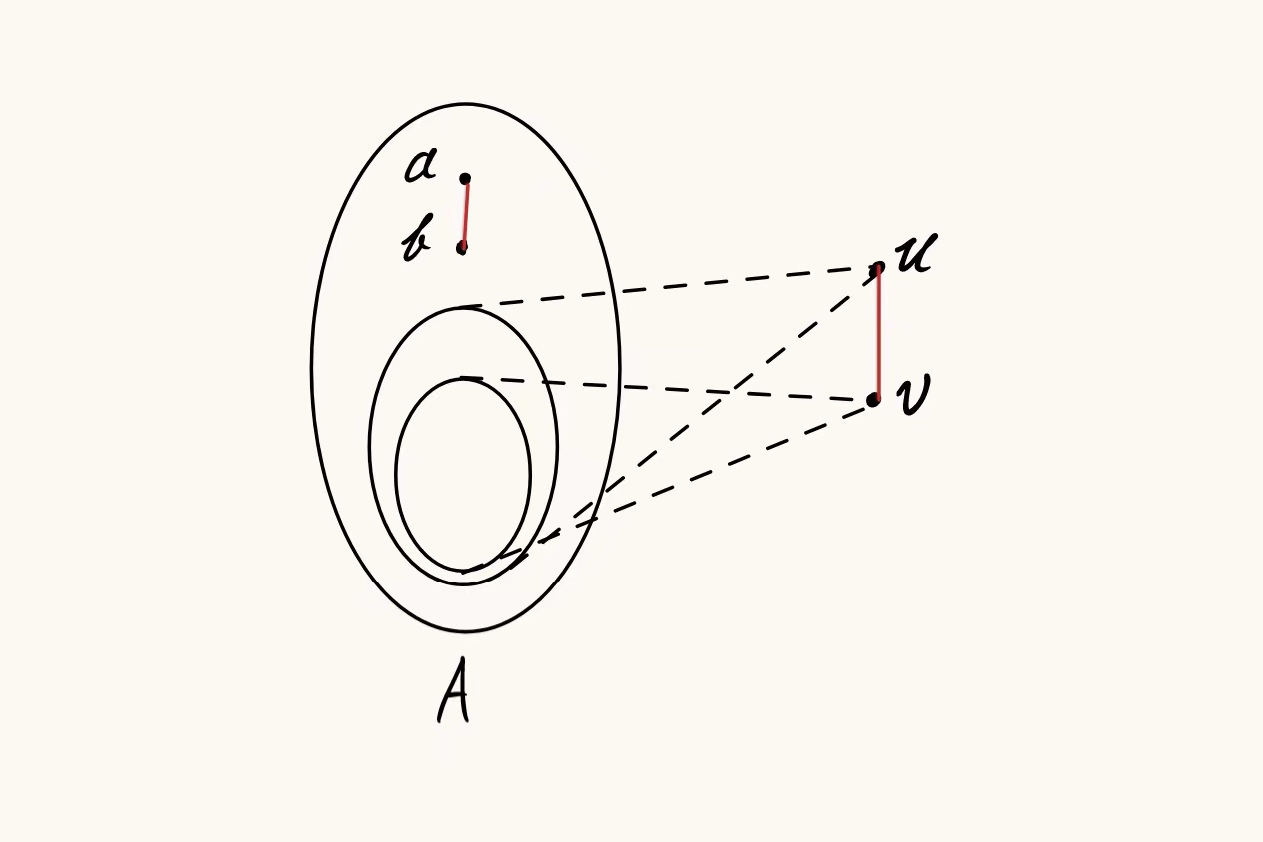
\includegraphics[width=0.45\textwidth]{pic/g2.jpg}
            %\caption{\textit{Schematic diagram of Hall effect}}\label{fig1}
        \end{figure}
    \end{proof}
    
    In proposition\eqref{p2}, we have checked that the relation between neighborhoods of two adjacent vertices is a containment relation. We then check whether they can be the same.

    \begin{prop}\label{p3}
        Neighborhoods of adjacent vertices in $B$ are not equal, i.e. $N_A(v)\neq N_A(w)$        
    \end{prop}

    \begin{proof}
        Suppose $N_A(v)=N_A(w)$, then by \textbf{Proposition}\eqref{p1}, we know that $v$ and $u$ are adjecent to every vertex in $A-\{k\}$. Thus $(A-\{k\})\cup\{u,v\}$ is a larger clique, which gives a contradiction to our assumption of $A$.
    \end{proof}
    
    \begin{corollary}\label{c1}
        For two adjacent vertices in $B$, there is exactly one of them, denoted by $u$, such that $\deg_A(u)=n-1$. (Here the "$\deg_A(u)$" means the number of vertices in $A$ that is adjacent to $u$)
    \end{corollary}

    %a graph
    
    With the help of \textbf{Corollary}\eqref{c1}, we could find some important information about the structure of $B$. An easy observation is that there would not be $C^3$ in $B$. Consider $uvwu$ a $C^3$, without losing generality, we may assume that $\deg_A(u)=n-1$, then $\deg_A(v),\ \deg_A(w)<n-1$. However, $v$ and $w$ are adjacent, which will give a contradiction to \textbf{Corollary}\eqref{c1}. Inspired by the observation above, we may find that any odd cycle would not be an induced subgraph of $B$.

    \begin{figure}[h!]%靠文字内容的右侧
        \centering
        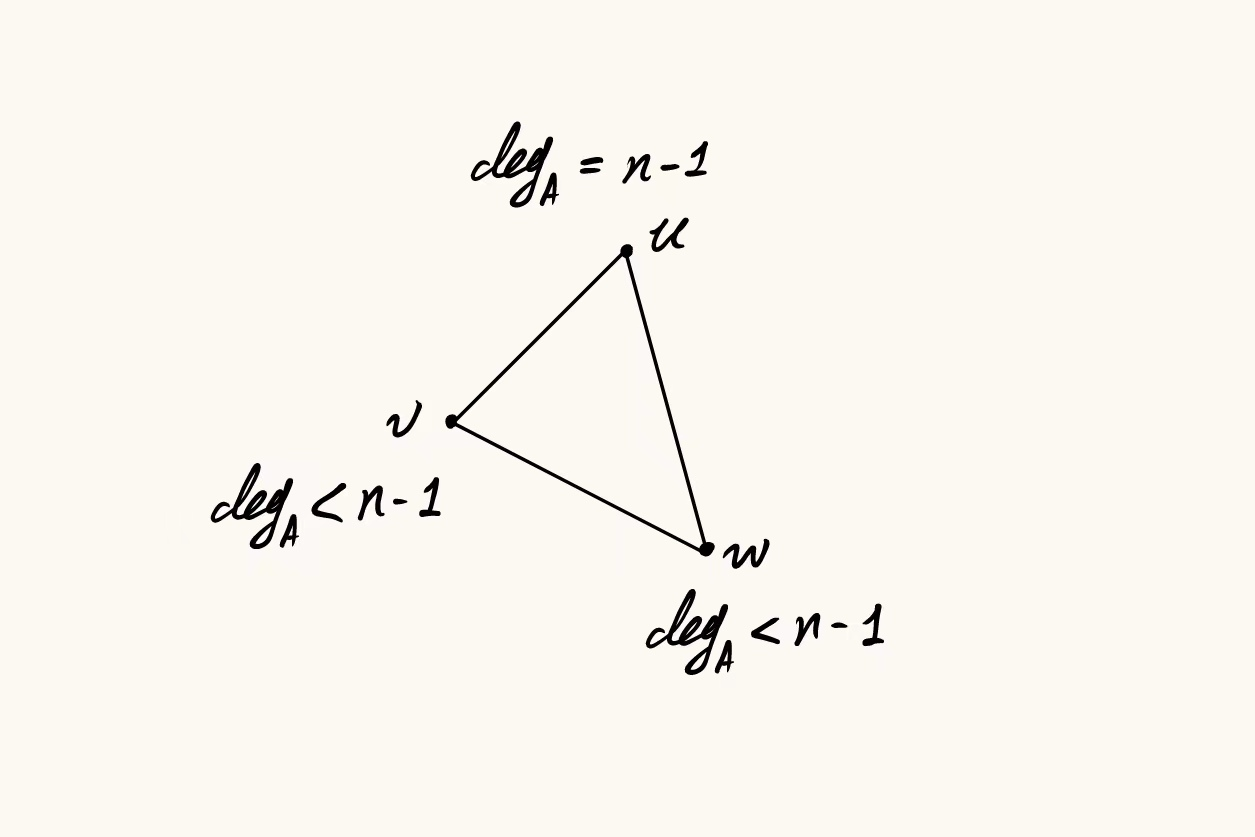
\includegraphics[width=0.45\textwidth]{pic/g3.jpg}
        %\caption{\textit{Schematic diagram of Hall effect}}\label{fig1}
    \end{figure}

    \newpage
    
    \begin{prop}
        $B$ is a bipartite graph.
    \end{prop}    
    
    \begin{proof}
        To show that $B$ is a bipartite graph, we may show that $C^{2n-1}$ is not embedded in $B$. One could try to prove it by contradiction. Assume that there is an odd cycle $u_1u_2\ldots u_{2n-1}u_1$ in $B$. Without losing generality, assume $\deg_A(u_1)=n-1$, then we know that $\deg_A(u_2)<n-1$. By induction, one could prove that $$\forall k\in\{1,2,\ldots,n\}\ \big(\deg_A(u_{2k-1})=n-1\big)$$
        However, $u_1$ and $u_{2n-1}$ are adjacent and they both have the same neighbors in $A$, which gives a contradiction. Thus $B$ is a bipartite.
    \end{proof}

    %a graph
    \begin{figure}[h!]%靠文字内容的右侧
        \centering
        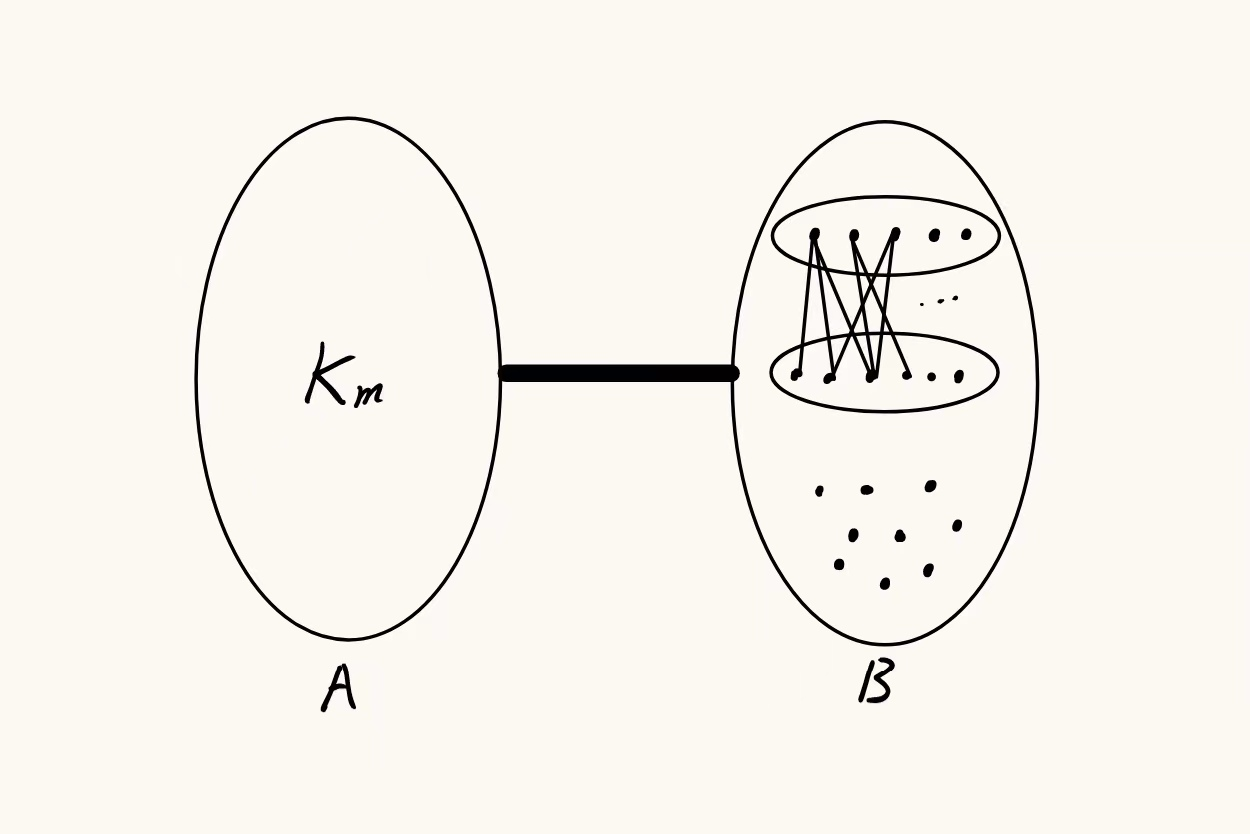
\includegraphics[width=0.45\textwidth]{pic/g4.jpg}
        %\caption{\textit{Schematic diagram of Hall effect}}\label{fig1}
    \end{figure}
    Since the bipartite is also $\text{Free}(2K^2,\, C^4)$, one could also find that the bipartite would have the following form. Note that the length of the path in the bipartite would not be larger than 3. Otherwise, we may find a $2K^2$ embedding in it.
    \begin{figure}[h!]%靠文字内容的右侧
        \centering
        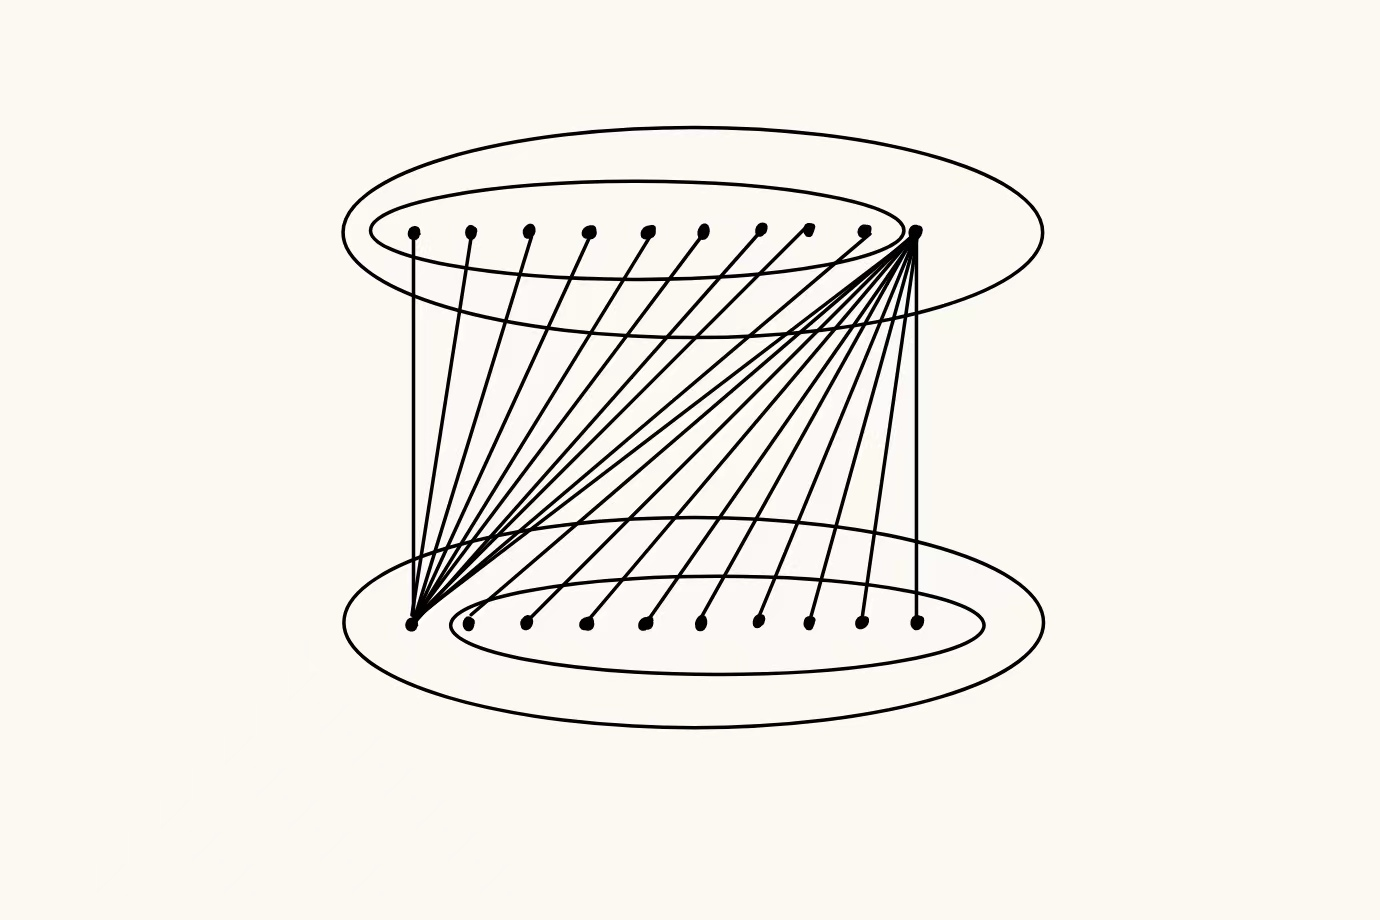
\includegraphics[width=0.4\textwidth]{pic/g5.jpg}
        %\caption{\textit{Schematic diagram of Hall effect}}\label{fig1}
    \end{figure}
    %a graph

    One would be curious about whether vertices of bipartite who have $n-1$ neighborhoods in $A$ have the same neighborhood.

    \begin{prop}
        In the bipartite in $B$, those non-independent vertices $u$ and $v$ with $\deg_A(u)=\deg_A(v)=n-1$ have the same neighbors.
    \end{prop}

    \begin{proof}
        Suppose $\deg_A(u)=\deg_A(v)=n-1$ and $N_A(u)\neq N_A(v)$, there exists a vertex $w$ in $B$ adjacent to both of them since the longest path in the bipartite is $P^3$, then
        \begin{equation*}
            \exists u'\in N_A(u)-N_A(v)\,\exists v'\in N_A(v)-N_A(u)\ \big(wuu'v'vw \text{ is a } C^5\big)
        \end{equation*}
        which gives a contradiction to $G\in\text{Free}\{2K^2,\,C^4,\,C^5\}$.
        \begin{figure}[h!]%靠文字内容的右侧
        \centering
        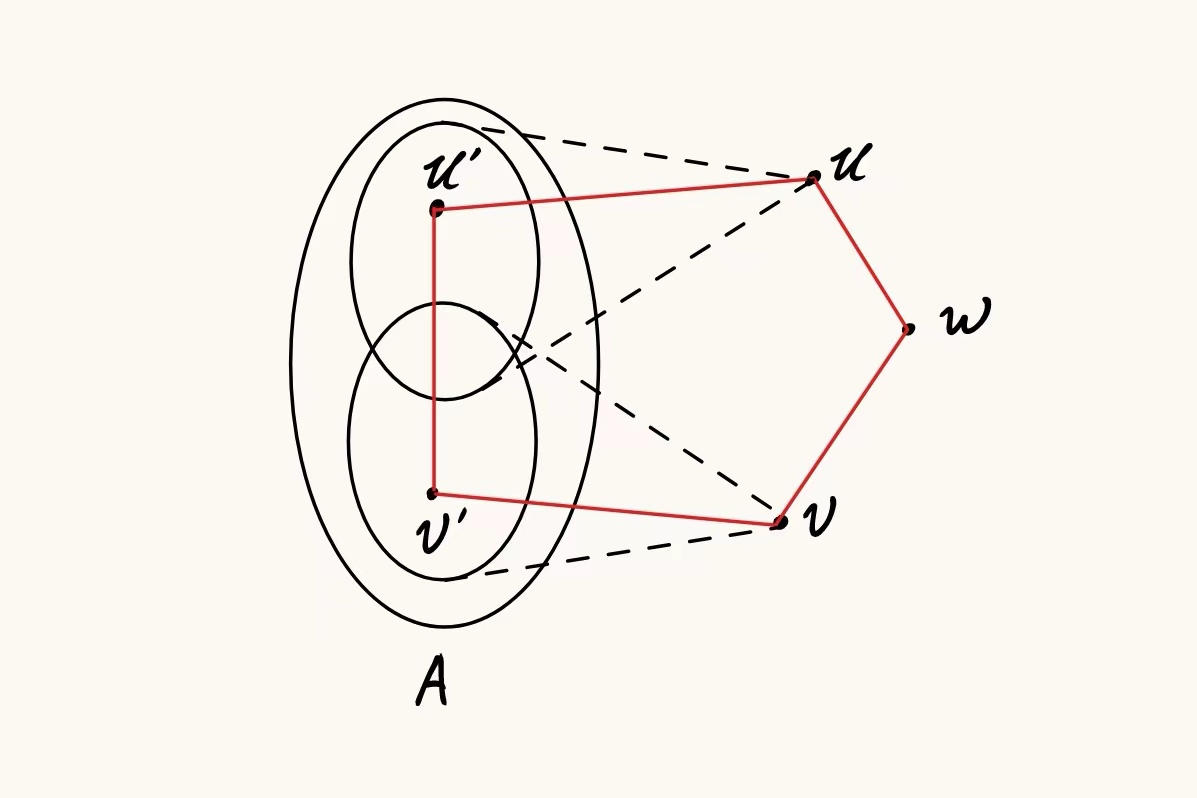
\includegraphics[width=0.4\textwidth]{pic/g6.jpg}
        %\caption{\textit{Schematic diagram of Hall effect}}\label{fig1}
    \end{figure}
    \end{proof}

    With the restriction to neighbors of vertices in the bipartite in $B$, one would find that it is impossible to have more than one $u$ such that $\deg_A(u)=n-1$.

    \begin{prop}
        Each vertex $v$ with $\deg_A(v)<n-1$ would only adjacent to one vertex $u$ with $\deg_A(u)=n-1$.
    \end{prop}

    \begin{proof}
        Suppose that $v\in B$ is adjacent to vertices $u_1,\,u_2$ such that $\deg_A(v)<n-1$ and thus $\deg_A(u_1)=\deg_A(u_2)=n-1$. Then take $w\in N_A(u_1)-N_A(v)$, one may find that $wu_1vu_2$ forms a $C^4$. Thus there would not be more than one vertex $v$ with $\deg_A(v)=n-1$.
        \begin{figure}[h!]%靠文字内容的右侧
        \centering
        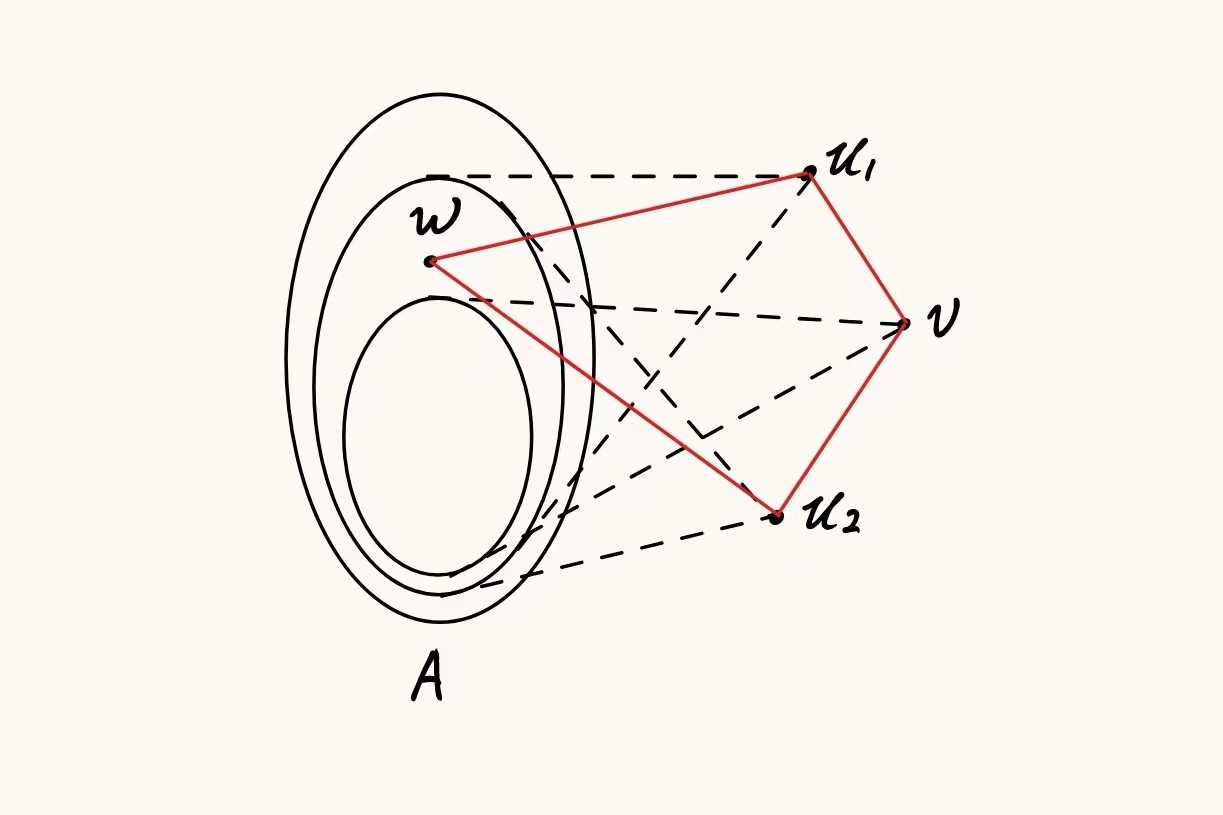
\includegraphics[width=0.4\textwidth]{pic/g7.jpg}
        %\caption{\textit{Schematic diagram of Hall effect}}\label{fig1}
    \end{figure}
    \end{proof}

    In our graph, one may find that there would only be one vertex in the bipartite (not an independent vertex) with $\deg_A$ being $n-1$. Denote such vertex by $p$.

    \begin{figure}[h!]%靠文字内容的右侧
        \centering
        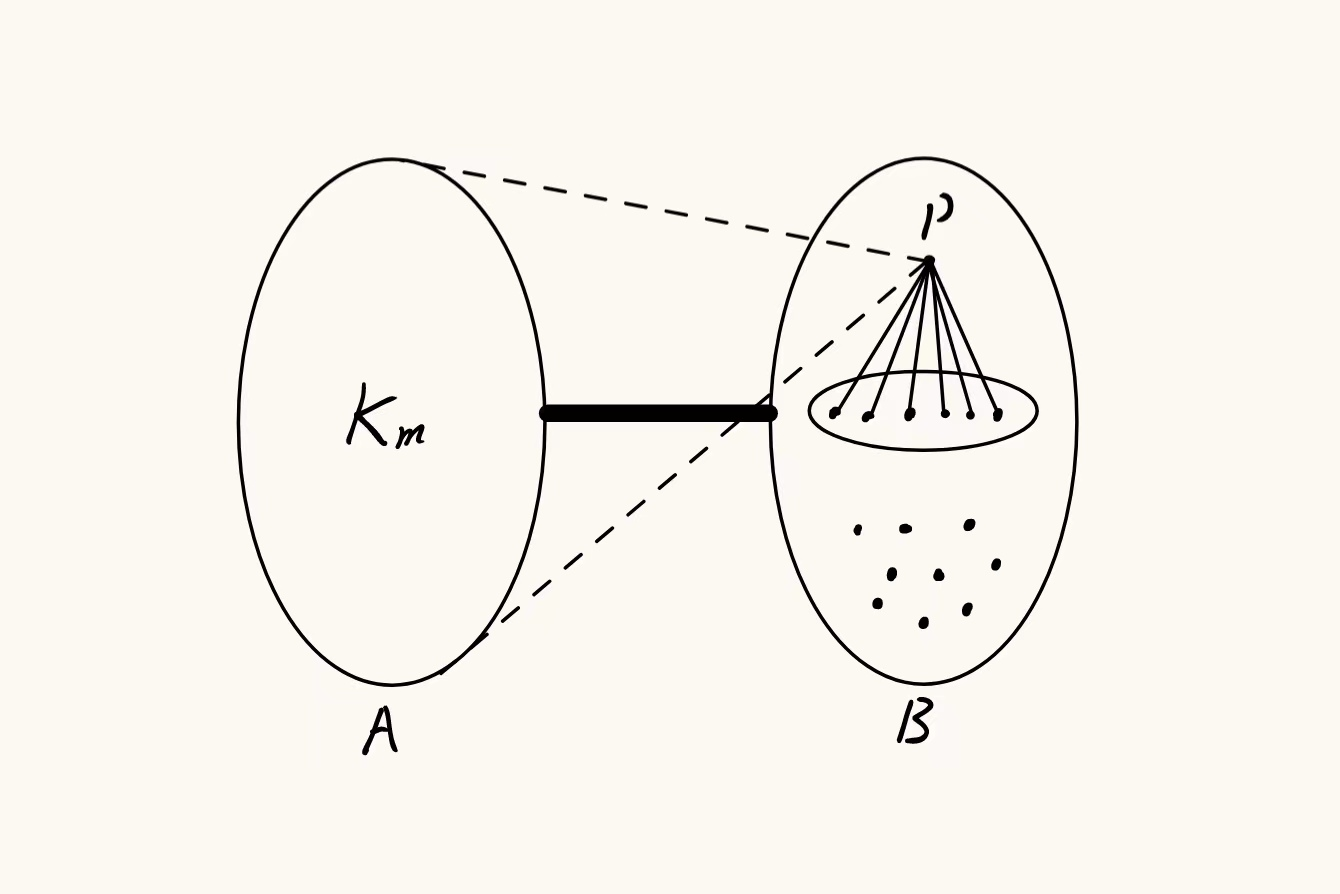
\includegraphics[width=0.4\textwidth]{pic/g8.jpg}
        %\caption{\textit{Schematic diagram of Hall effect}}\label{fig1}
    \end{figure}
    
    Having discussed the properties of the bipartite graph, we need to find some important information about those independent vertices in $B$
\newpage
    \begin{prop}
        The vertices independent in $B$ would not be adjacent to $k$.
    \end{prop}

    \begin{proof}
        Suppose $w\in B$ with $N_B(w)=\emptyset$ and $kw$ is an edge. Let $u$ be a vertex adjacent to $p$. Then one may find that $kw+pu$ is a $2K^2$. Which gives a contradiction to $G\in\text{Free}\{2K^2,\,C^4,\,C^5\}$.
        \begin{figure}[h!]%靠文字内容的右侧
        \centering
        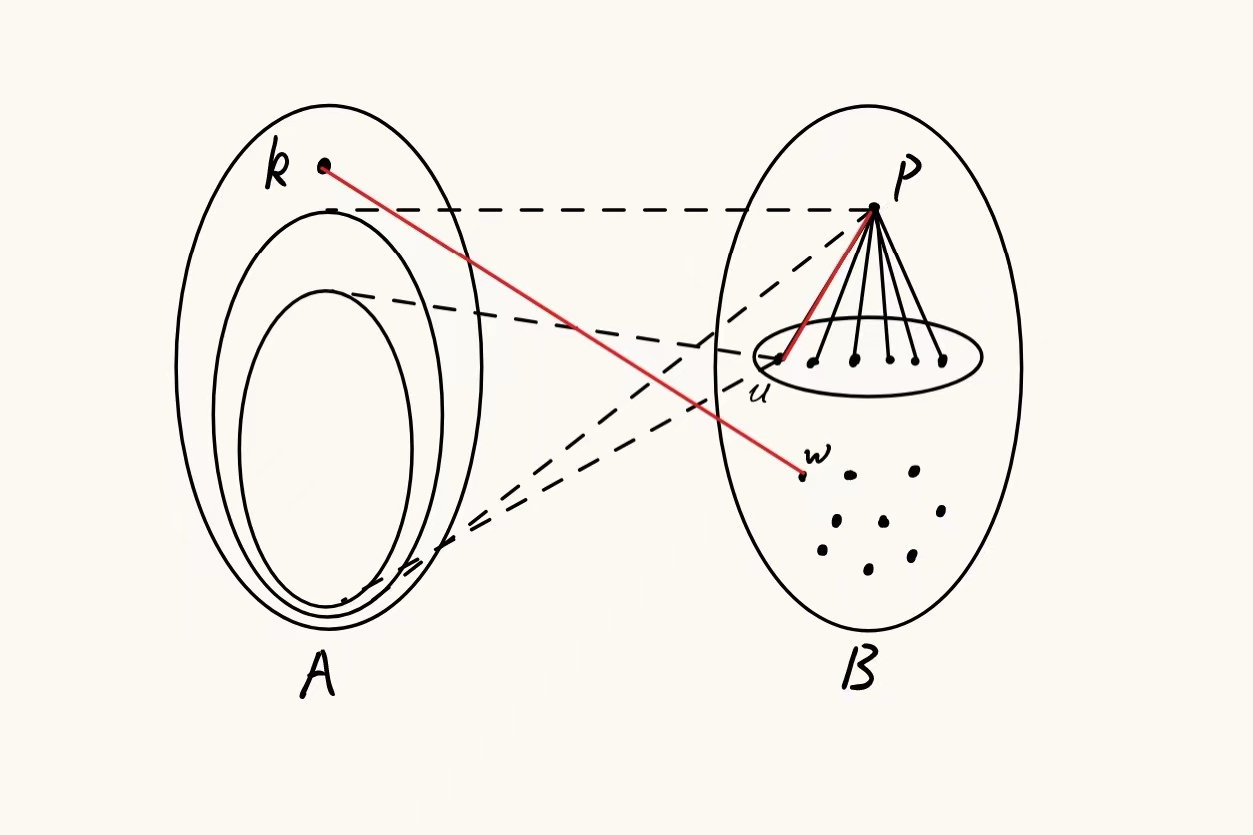
\includegraphics[width=0.45\textwidth]{pic/g9.jpg}
        %\caption{\textit{Schematic diagram of Hall effect}}\label{fig1}
    \end{figure}
    \end{proof}

    Remove $k$ into $B$ and $p$ into $A$, we would split the graph into a clique and an independent set.
    \begin{figure}[h!]%靠文字内容的右侧
        \centering
        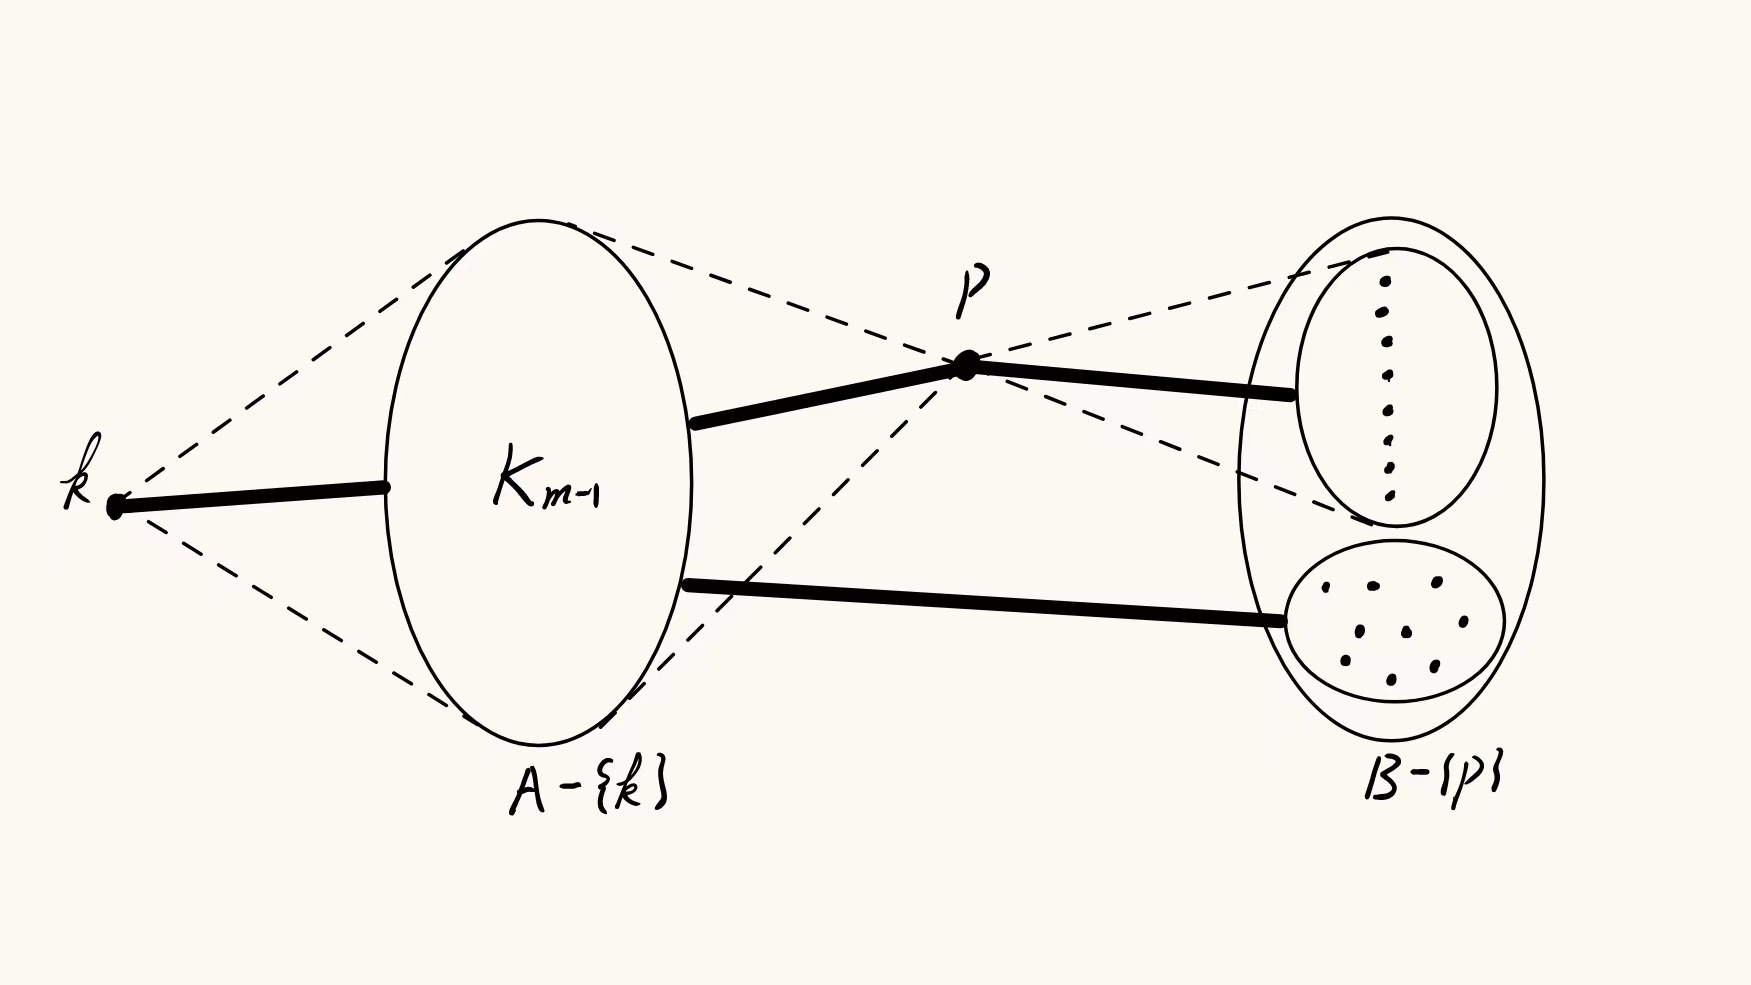
\includegraphics[width=0.45\textwidth]{pic/g10.jpg}
        %\caption{\textit{Schematic diagram of Hall effect}}\label{fig1}
    \end{figure}
\end{document}
    